\chapter{实验结果与分析}
\label{cha:res}

实验将抓取的高性能应用的IO Trace通过映射和垃圾回收机制转换为对开放通道SSD内部结构操作,并使用liblightnvm对其进行直接读写,最后通过IO吞吐量,单次IO的延迟和速率,映射表修改开销等指标评价优化方法的优劣。此外,实验还研究了不同优化方法下剩余空间大小对IO性能的影响,以及超级块方法中超级块参数的影响。

\section{实验环境}
由于硬件条件限制,本章中所有实验均在开放通道SSD的模拟器上进行。因此,下文的"硬件环境"包括运行模拟器的设备的硬件环境,模拟器以及模拟出的开放通道SSD的基本参数。下文的"软件环境"包括模拟器使用的Linux内核版本与相关用户态库的信息。
\subsection{硬件环境}
实验使用一台Linux服务器运行模拟器,服务器的CPU为Intel(R) Xeon(R) CPU E5-2620 v2 @ 2.10GHz,内存大小16GB。模拟器使用https://github.com/DFC-OpenSource/qemu-ox 提供的支持模拟开放通道SSD的qemu虚拟机。除特殊说明外,实验使用的模拟开放通道SSD设备基本信息如下表:
\begin{table}[htb]
    \centering
    \begin{minipage}[t]{0.8\linewidth}
    \caption[开放通道SSD的基本信息]{开放通道SSD的基本信息}
    \label{tab:res_ocssd_geo}
      \begin{tabularx}{\linewidth}{cY}
        \toprule[1.5pt]
        {\heiti 参数名} & {\heiti 数值} \\\midrule[1pt]
        Channel数量 & 8\\
        每个Channel的Lun数量 & 4\\
        每个Lun的Block数量 & 64\\
        每个Block的Page数量 & 8\\
        每个Page的Sector数量 & 4\\
        Plane数量 & 2\\
        每个Sector能够容纳的数据量 & 4096 Byte\\
        每个Page能够容纳的数据量 & 32768 Byte\\ 
        \bottomrule[1.5pt]
    \end{tabularx}
\end{minipage}
\end{table}
\subsection{软件环境}
模拟器运行的Linux内核版本为4.17.0,编译时打开了CONFIG\_BLK\_DEV\_NVME,CONFIG\_NVM,CONFIG\_NVM\_DEBUG,CONFIG\_NVM\_PBLK选项以提供对开放通道SSD的驱动支持。实验使用的用于直接操作开放通道SSD设备的用户态库liglightnvm版本为master@ba201ca。

\section{IO吞吐量}
下图展示了不同优化方法重放高性能应用IO Trace时的IO吞吐量。
\begin{figure}[H]
    \centering
    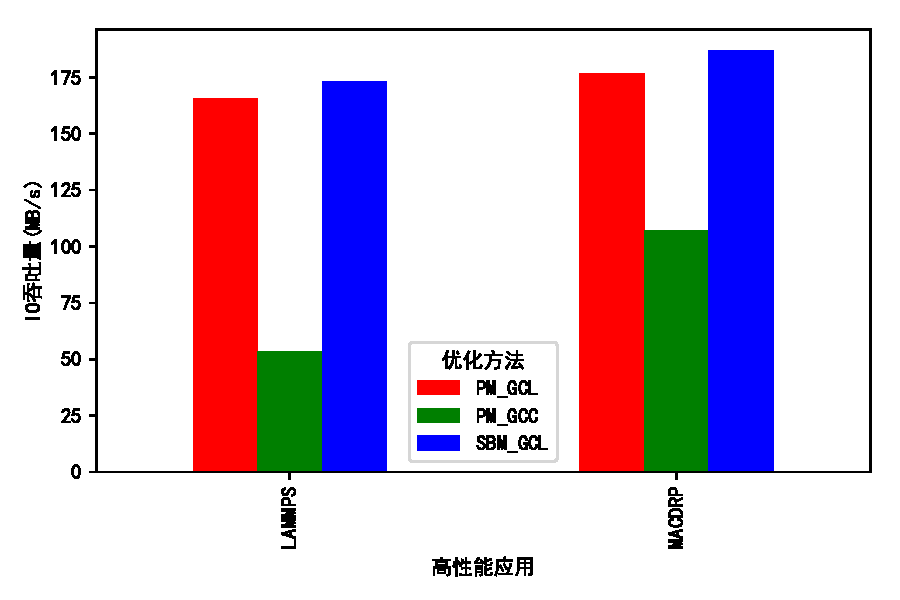
\includegraphics[width=0.8\textwidth]{iothroughput.pdf}
    \caption{不同优化方法的IO吞吐量}
    \label{fig:res_iototal}
\end{figure}

\begin{table}[htbb]
    \centering
    \begin{minipage}[t]{0.8\linewidth}
    \caption[不同优化方法的IO吞吐量(MB/s)]{不同优化方法的IO吞吐量(MB/s)}
    \label{tab:res_iototal}
    \begin{tabularx}{\linewidth}{cYYY}
        \toprule[1.5pt]
        \multirow{2}{*}{\heiti{高性能应用}} & \multicolumn{3}{c}{\heiti{优化方法}}  \\ \cmidrule(l){2-4} 
                     & PM\_GCL & PM\_GCC & SBM\_GCL \\ \midrule[1pt]
                     LAMMPS &65.448&53.217    & \textbf{173.116}    \\
                     MACDRP    & 176.768 &107.184    & \textbf{186.747}    \\ \bottomrule[1.5pt]
        \end{tabularx}
    \end{minipage}
\end{table}

\begin{figure}[H]
    \centering
    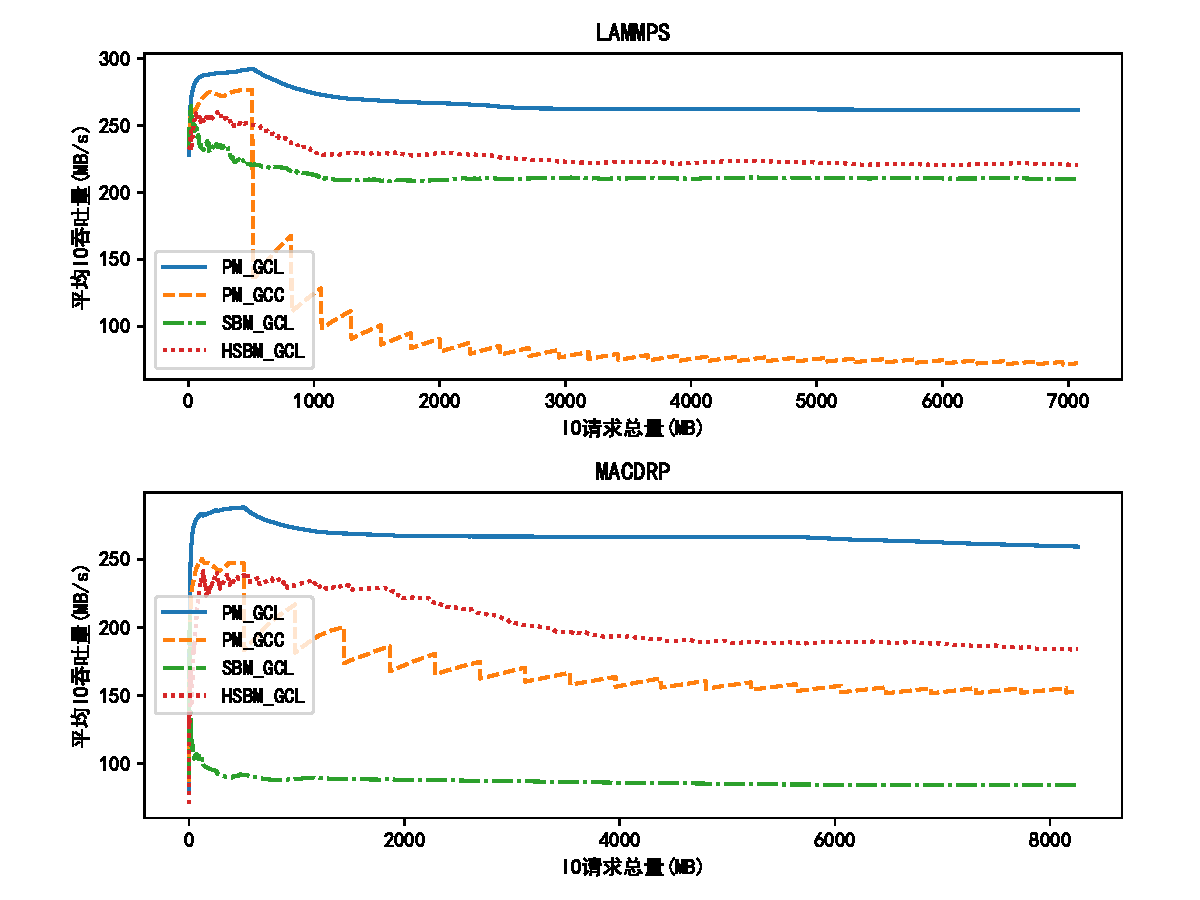
\includegraphics[width=0.8\textwidth]{avgiothp.pdf}
    \caption{平均IO吞吐量在重放过程中随IO请求总量的变化}
    \label{fig:res_ioavg}
\end{figure}

\begin{figure}[H]
    \centering
    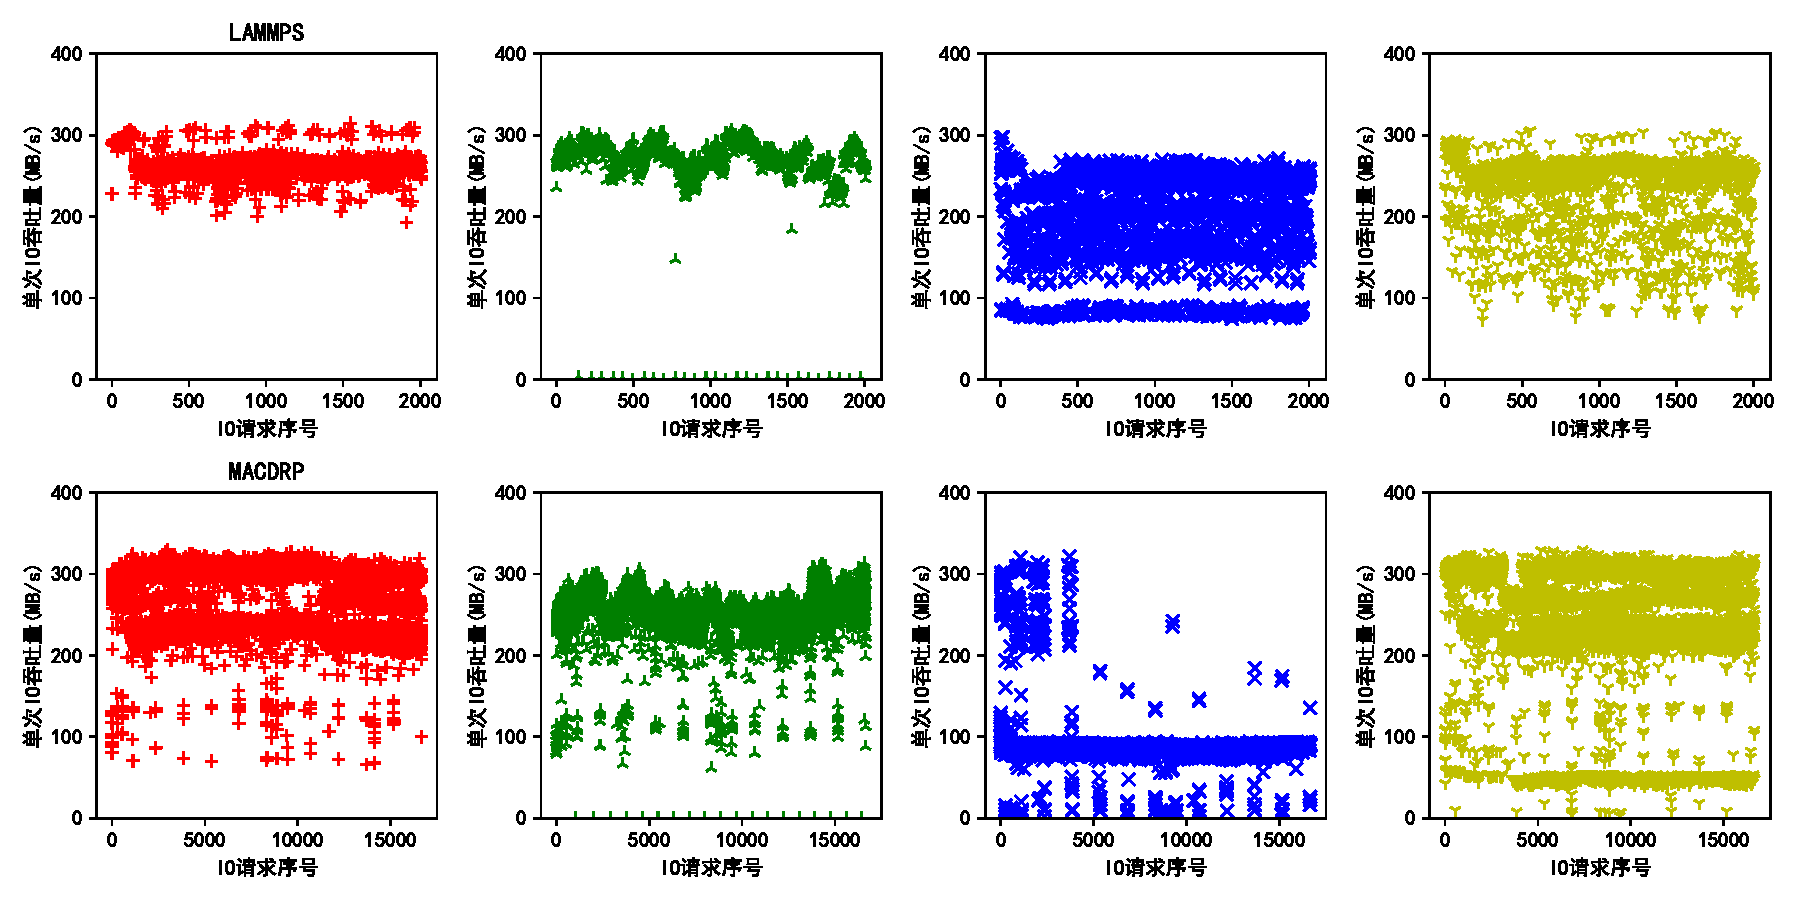
\includegraphics[width=0.8\textwidth]{singleiothp.pdf}
    \caption{不同优化方法在重放过程中的单次IO吞吐量}
    \label{fig:res_isingle}
\end{figure}

\section{映射表开销}

\begin{figure}[H]
    \centering
    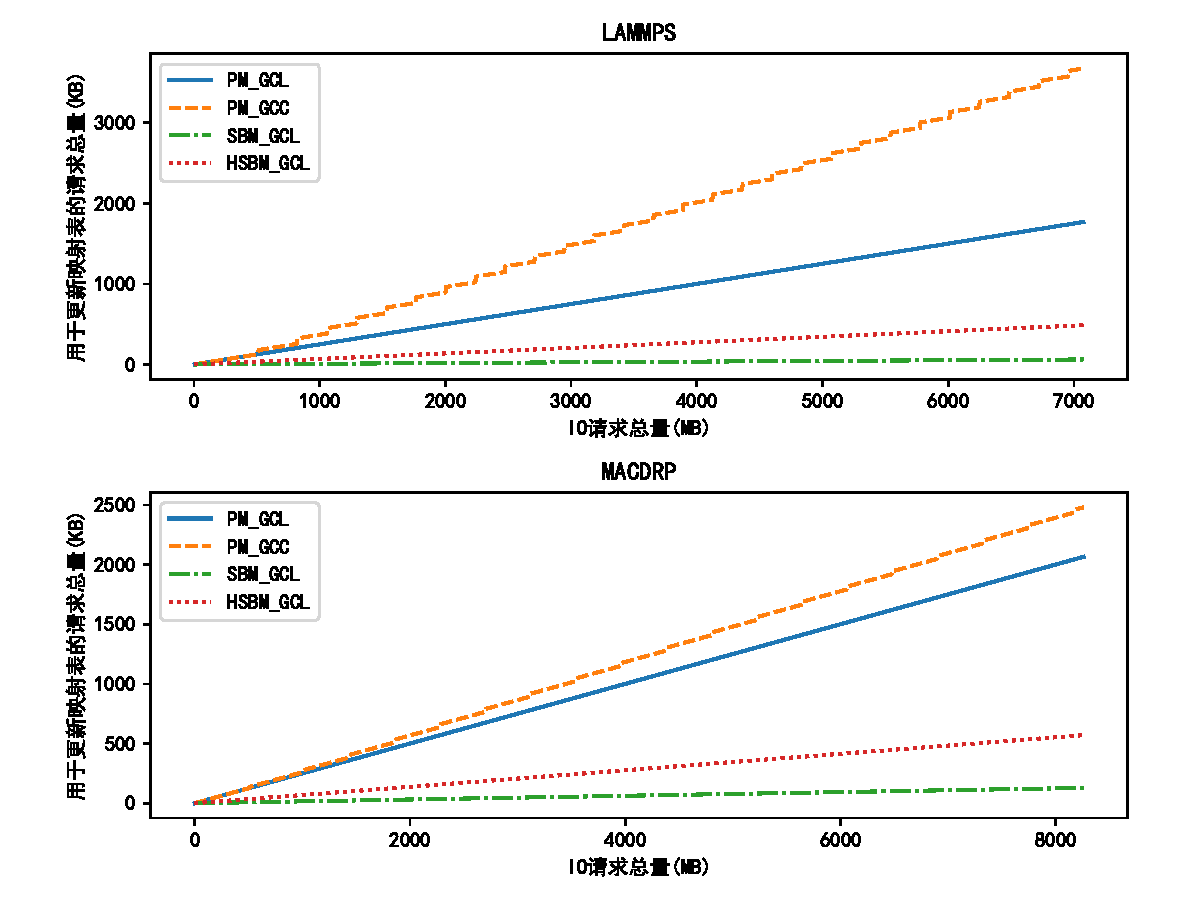
\includegraphics[width=0.8\textwidth]{mapupdateio.pdf}
    \caption{用于更新映射表的请求总量在重放过程中随IO请求总量的变化}
    \label{fig:res_mapupdate}
\end{figure}

\section{擦除次数与写放大系数}

\begin{figure}[H]
    \centering
    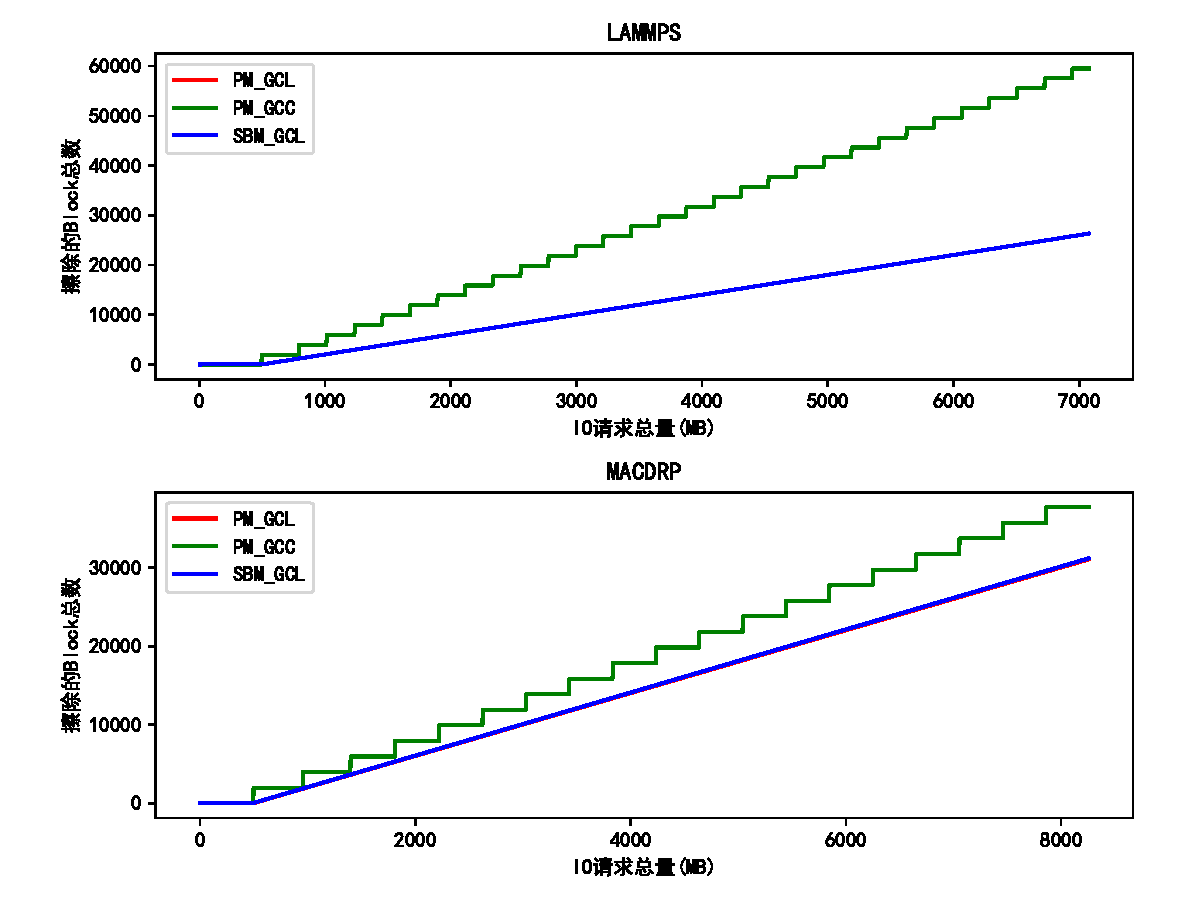
\includegraphics[width=0.8\textwidth]{eraseblk.pdf}
    \caption{擦除的Block数在重放过程中随IO请求总量的变化}
    \label{fig:res_writeamp}
\end{figure}

\begin{figure}[H]
    \centering
    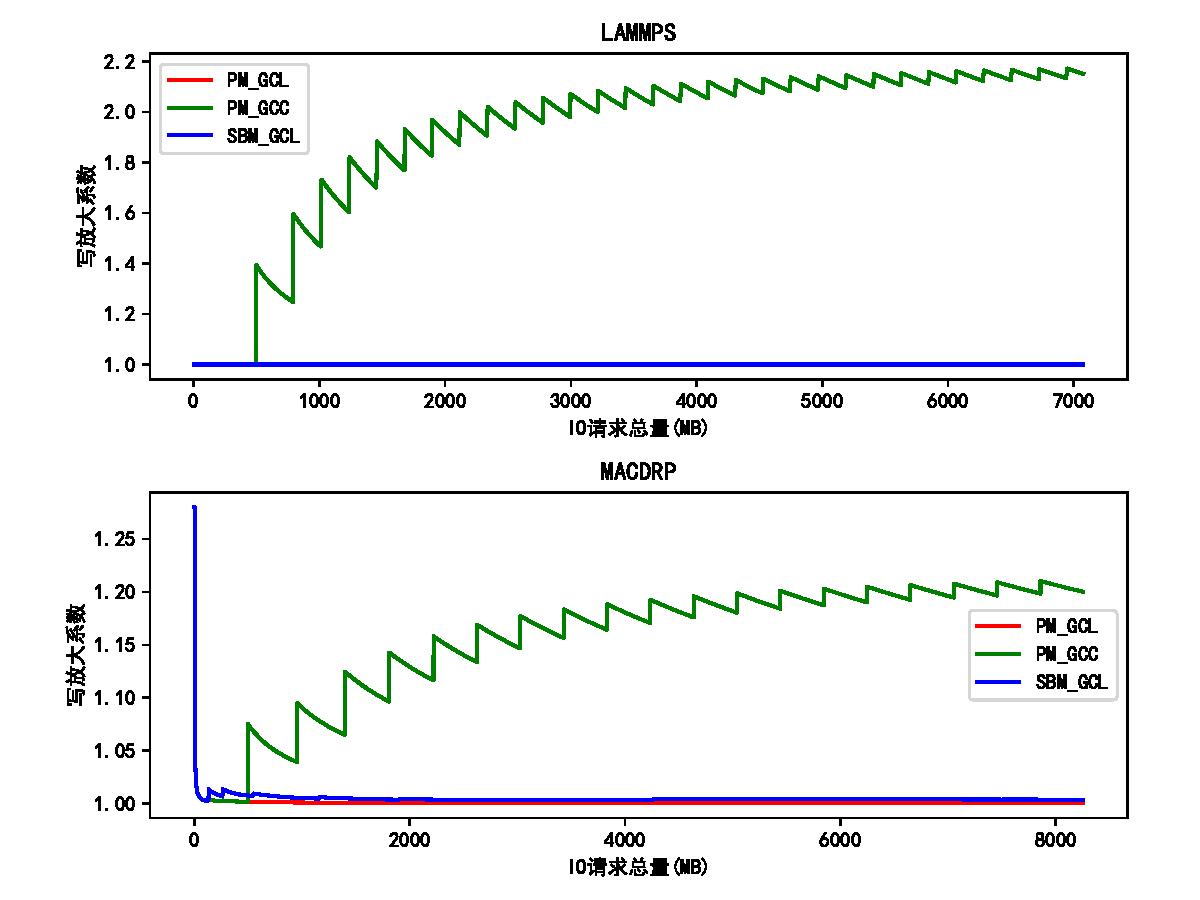
\includegraphics[width=0.8\textwidth]{writeampio.pdf}
    \caption{写放大系数在重放过程中随IO请求总量的变化}
    \label{fig:res_writeamp}
\end{figure}

\section{负载均衡}

\begin{figure}[H]
    \centering
    \subcaptionbox{重放LAMMPS时的负载分布}
      {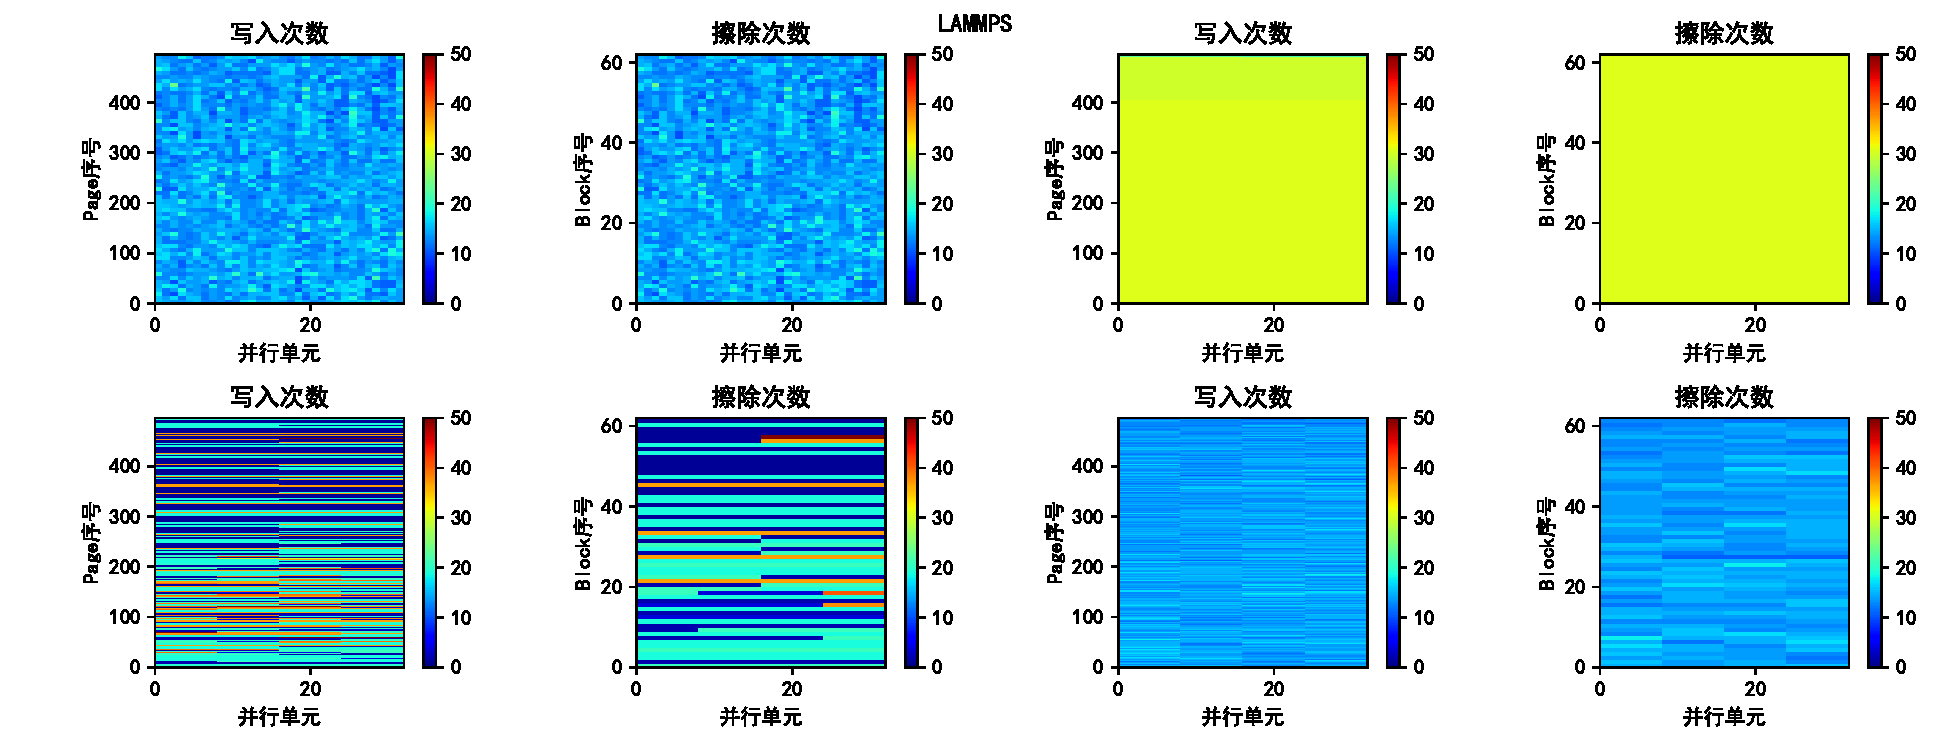
\includegraphics[width=0.8\textwidth]{heatmap_lammps.pdf}}
    \vspace{4em}
    \subcaptionbox{重放MACDRP时的负载分布}
        {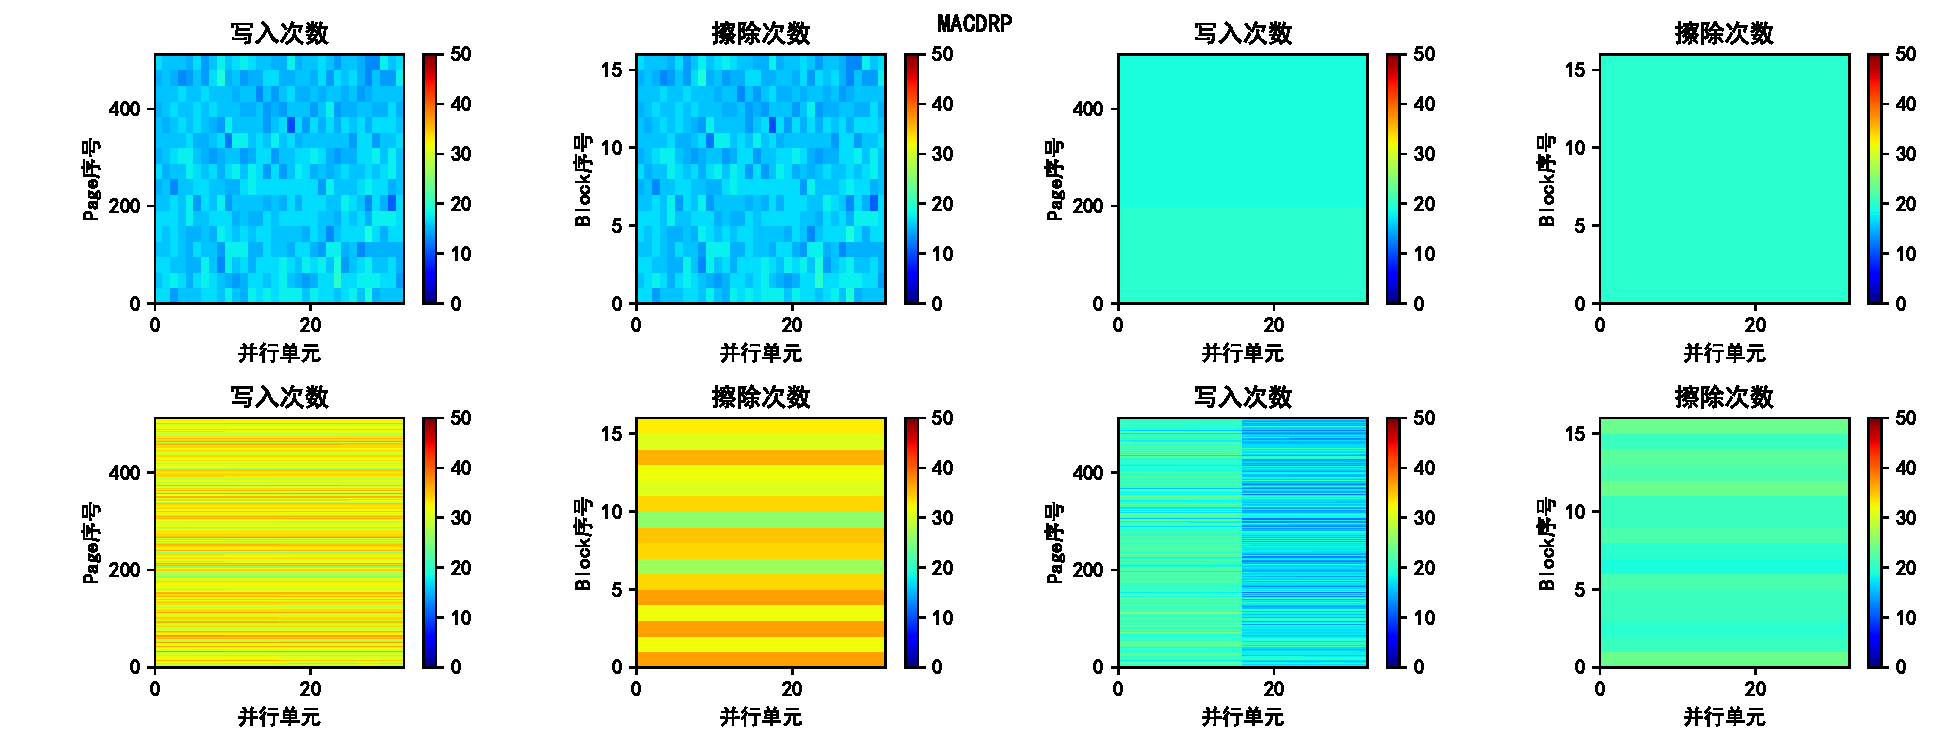
\includegraphics[width=0.8\textwidth]{heatmap_macdrp.pdf}}
    \caption{负载分布图}
    \label{fig:res_heatmap}
\end{figure}

\section{剩余空间的影响}

\begin{figure}[H]
    \centering
    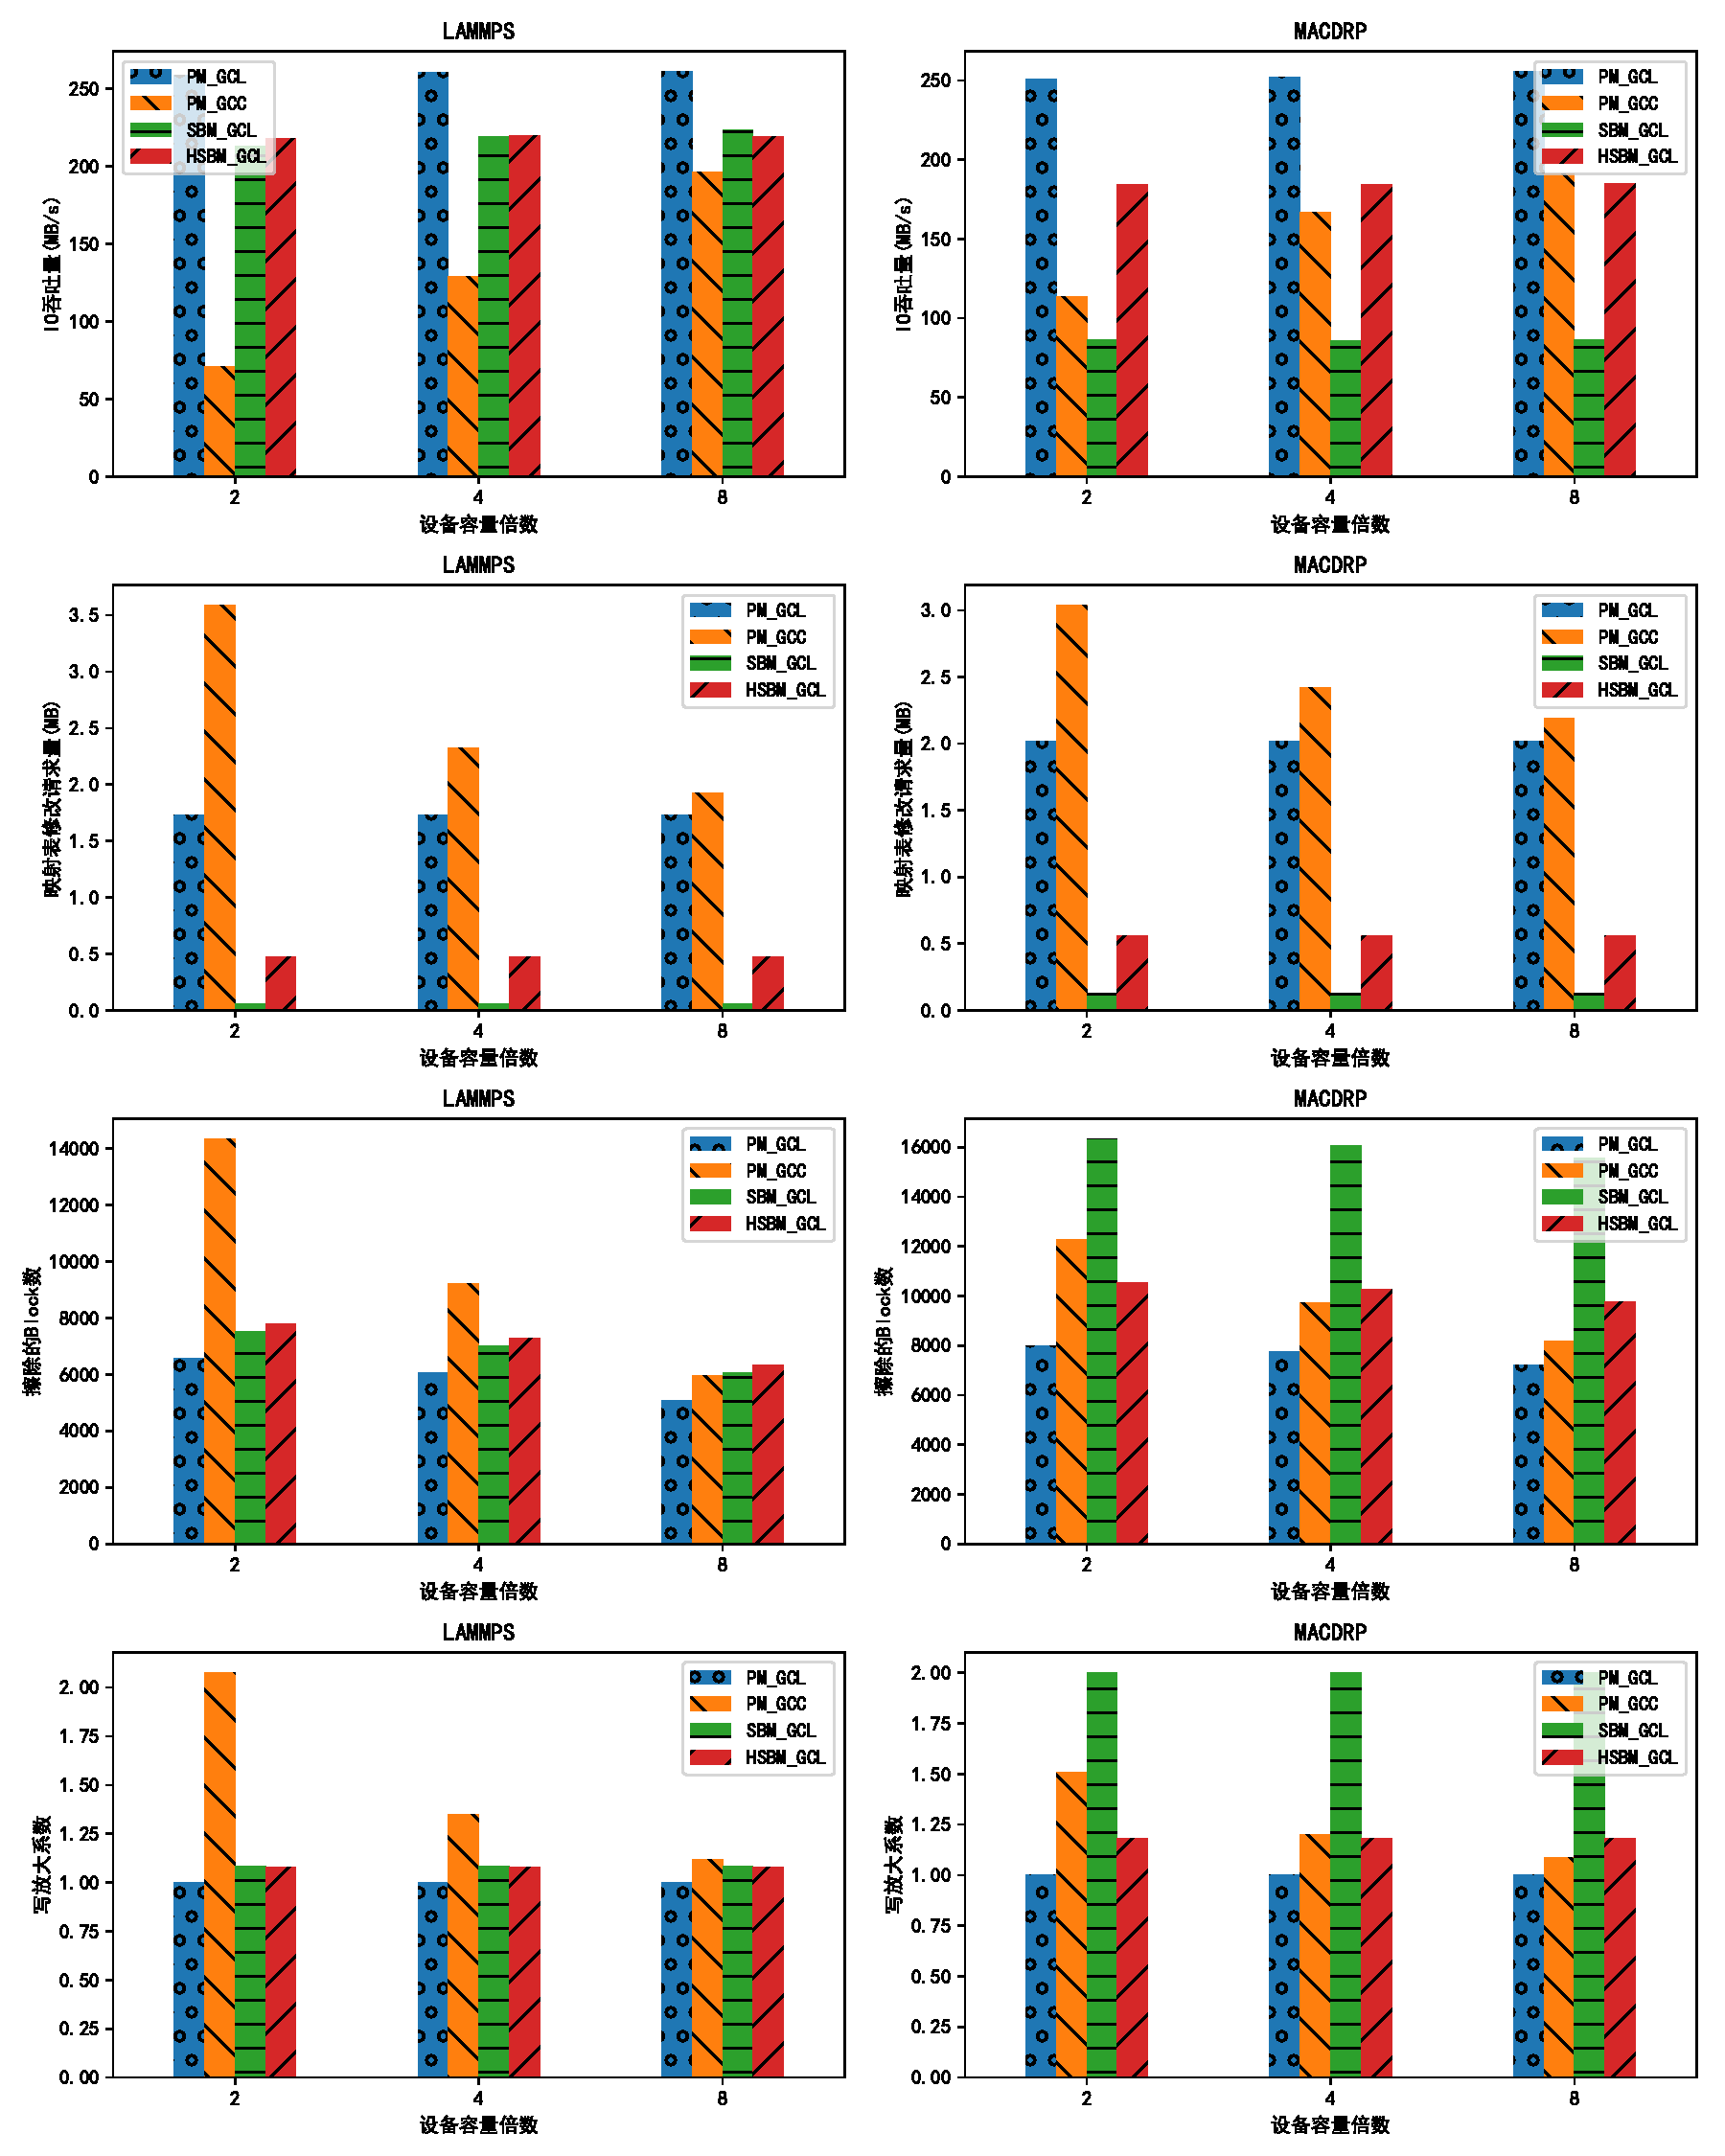
\includegraphics[width=0.8\textwidth]{disksize.pdf}
    \caption{剩余空间对各项性能指标的影响}
    \label{fig:res_disksize}
\end{figure}

\section{超级块大小的选择}

\begin{figure}[H]
    \centering
    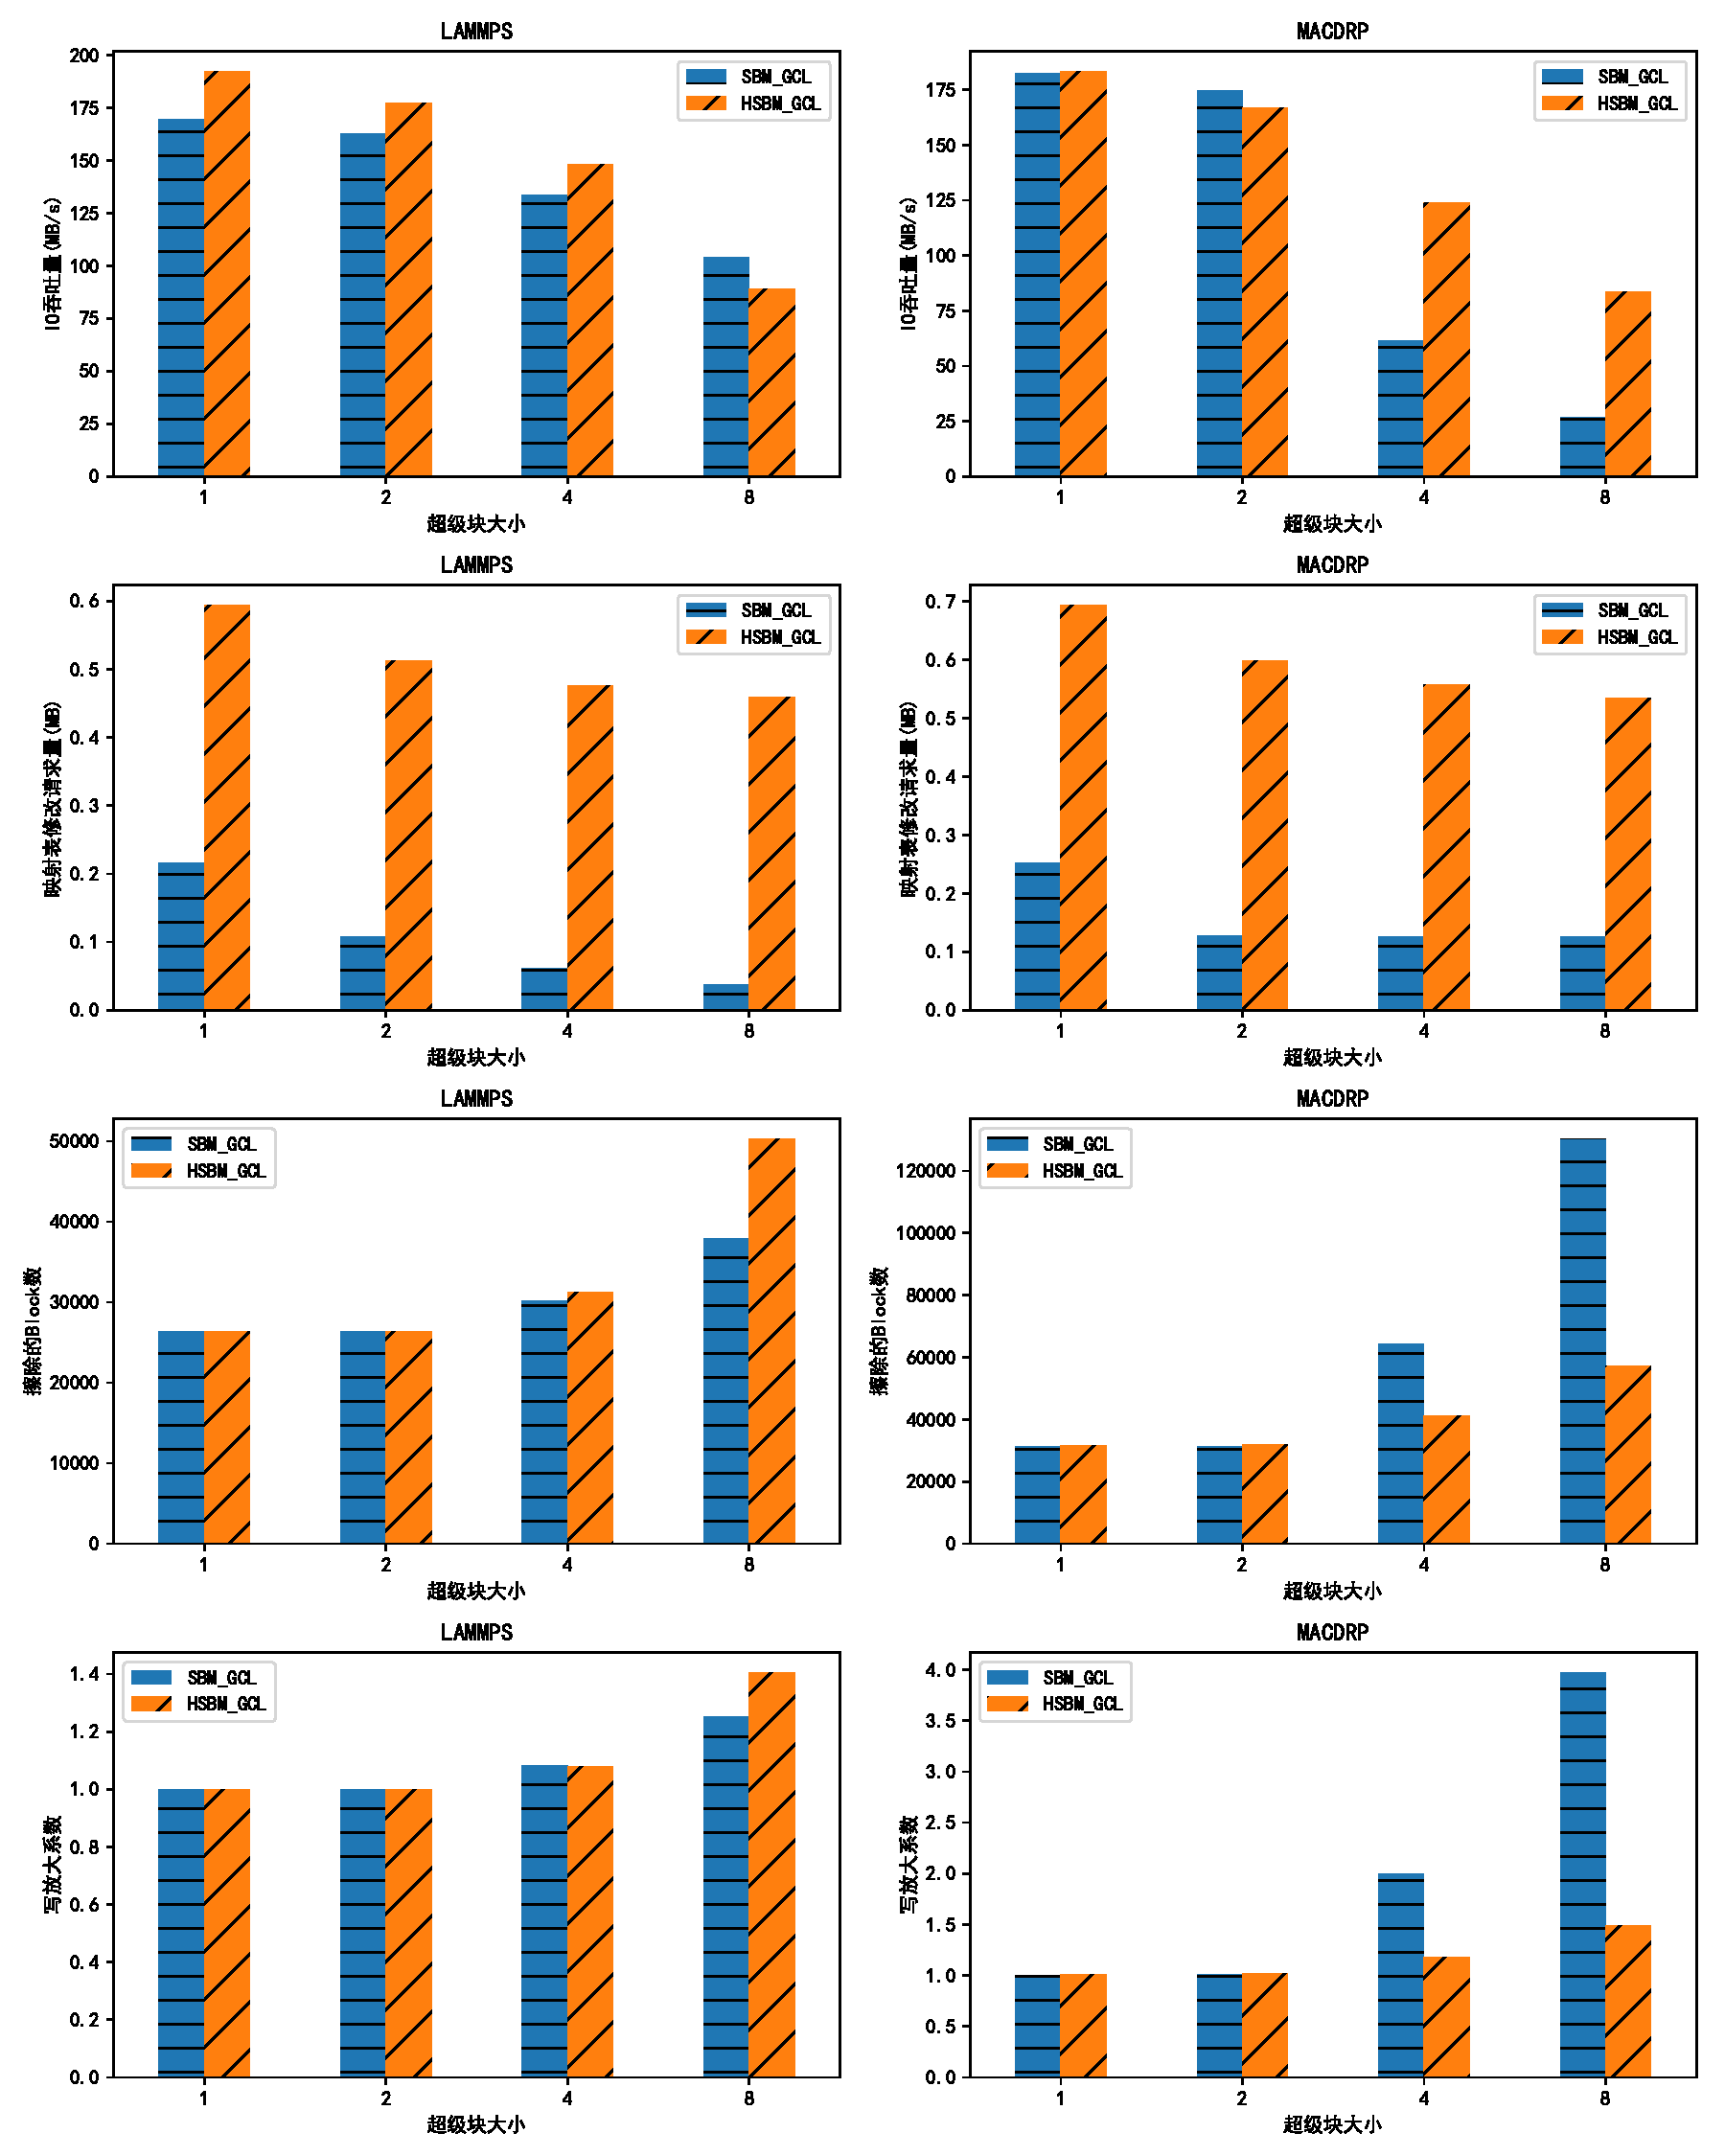
\includegraphics[width=0.8\textwidth]{sbsize.pdf}
    \caption{超级块大小对各项性能指标的影响}
    \label{fig:res_sbsize}
\end{figure}

\section{本章小结}